\documentclass{article}
\usepackage[utf8]{inputenc}

\title{Empowering local IT with open-source tools}
\author{Lauri Võsandi}
\date{January 2015}

\usepackage{natbib}
\usepackage{graphicx}
\usepackage{url}
\usepackage{tikz}

\begin{document}

\maketitle

\section{Introduction}

Can you take control over your IT with open-source tools?

empowerment literature
economic 
localization
marketing hype
economic interest of other to make it more complicated than it is

Up to now Linux-based operating system deployment has been
error prone, time-consuming process and usually specific to
a particular distribution of Linux.
Linux-based operating systems also have a long history
of being overly complex to set up for a novice computer user.
Even though Linux-based operating systems have made significant
progress on the servers
\footnote{Google and Amazon have successfully used open-source software
and commodity hardware to build enterprise grade cloud}
and embeddeded systems
\footnote{Android is the market leader in smartphones and it is composed of open-source components such as Linux},
the workstations and laptops have been left without attention.
%According to DistroWatch Ubuntu, ?? and ?? are the three most
%favored Linux distributions for end users.
In the major thesis technical solution to reduce
Linux-based operating system deployment time using
Btrfs filesystem is presented and in this paper the business aspects
of the solution and related services are discussed.


\section{Background}

Tiger's Leap (Tiigrihüpe) was a program announced
by president Lennart Meri in 1996 with the plan to heavily invest
in computers and network infrastructure in Estonia.
As part of Tiger Leap program schools procured IBM PC-s and
other equipment.
As part of Look@World (Vaata Maailma) program
various web applications were unrolled for schools such as
eKool (e-school) in 2002 which is used to keep track of student attendance.
This transformed a soviet country into an advanced paperless e-society.

It is common for western IT corporations to offer products
and services for developing countries at sub-nominal prices in order
to gain userbase
\footnote {viide MS lehele}.
Once the country has reached certain living standard the
pricing is adjusted accordingly.
As the users have been learning to use particular product,
reluctance to switch is increased due to training costs,
user fustration etc. 
%Most often organizations submit to paying
%licensing fees at significantly higher prices due to increased
%user discontent because of switch.
Starting from the end of 2013 Microsoft does not consider Estonia a
developing country anymore. The implication of the change was that
the Microsoft Windows and Microsoft Office license fees would rise
from current 6 EUR to 60 EUR per month per machine.
According to Ernst \& Young analysis Tallinn could save 490 000 EUR
within five years if they would give up Microsoft Office now.
Replacing Windows with Linux would save additional 210 000 EUR.
\cite{ernst-young-report}
This was the main motivation for Tallinn Education Department to try
out alternatives. As change from Microsoft Office to LibreOffice was
certain, replacing operating system was more questionable.

In March of 2014 Tallinn Education Board decided
to pilot Linux in five educational sinstitutions:
Mustamäe Upper Secondary School
\footnote{http://mg.edu.ee},
Tallinn Mahtra Primary School
\footnote{mahtra.tln.edu.ee},
Merivälja school
\footnote{meripohi.edu.ee},
Tallinn Mesimummu kindergarten
\footnote{mummula.net} and
Tallinn Tammetõru kindergarten
\footnote{1algtln.edu.ee}.
Procurement competition was won by Arvuti Traumapunkt OÜ
\footnote{http://atrauma.ee} and
Silver Püvi hired me to take care of setting up infrastructure servers.
Most of the work so far has been done remotely in conjunction with
local IT-support. Before the migration I had around seven years of
open-source hacking experience, however I never had experience with
remote management or centralized authentication.

In addition to financial aspects, the privacy concerns rised by
Edward Snowden in 2011
\footnote{bla}
pushed various governments to seek for alternatives
to relying on proprietary technology.
For instance use of Windows 8 has been banned in German governmental agencies
\footnote{\url{http://blog.legalsolutions.thomsonreuters.com/law-and-techology/german-government-bans-windows-8-use-nsa-spying-puts-american-companies-risk/}}.
Similariliy Indian Government mandates use of open-source technologies
in order to reduce total cost of ownership and to ensure
strategic control of e-Governance applications and systems
\footnote{\url{http://deity.gov.in/sites/upload_files/dit/files/policy_on_adoption_of_oss.pdf}}.

Thus, there is interest on political level, but due to lack
of technical competence contradicting decisions are made.



\section{Challenge}

Prior the project the author never had experience managing Linux based workstations.
The goal was to provide a platform which would be easier than current Windows
workstations.
In retrospective maintaining Linux-based and in fact
Windows workstations as well concerns several aspects:

\begin{itemize}
\item Provisioning - getting the initial software setup onto the computer
\item Updating - keeping the software up to date
\item Configuration management - adjusting configuration of various software components
\item Central authentication - keeping user accounts off the machines
\item Networked storage - keeping user files off the machines
\end{itemize}

The need for configuration management, central authentication
and networked storage was recognized immideately.


Puppet was chosen for configuration management due to it's
enterprise capabilities and vibrant community.
Foreman was used as Puppet web interface to provide
overview of the inventory.
Initially Puppet was used to also perform software updates, but
it turned out to be a bad idea because even though Ubuntu package
management performs well for most cases, there are still some
corner cases which may render the whole package management
system unusable.

\begin{figure}[!htb]
\centering
\scalebox{0.5}{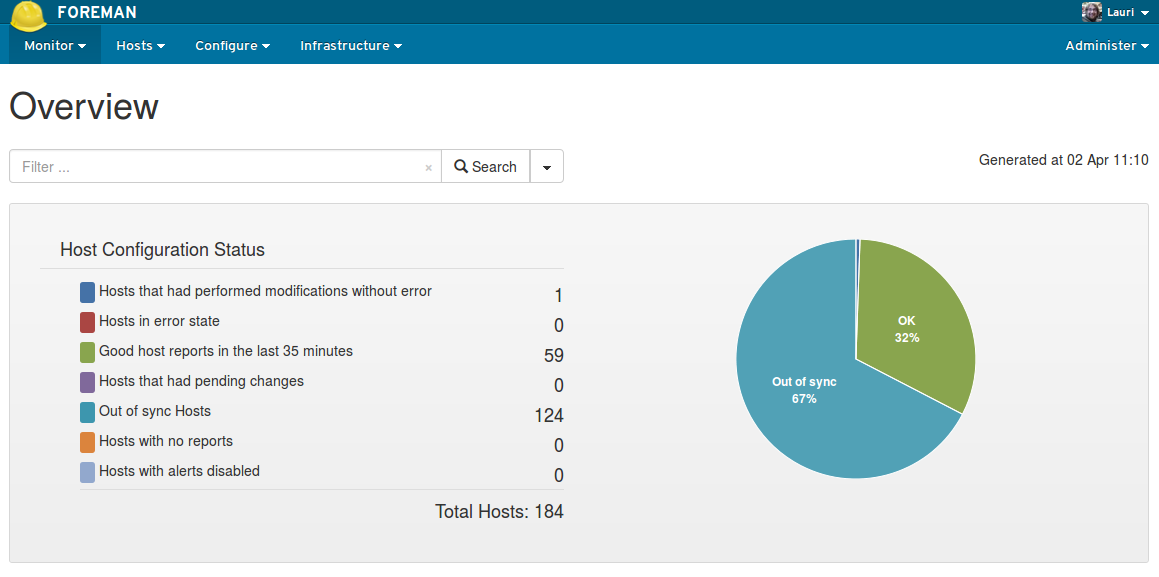
\includegraphics[scale=0.6]{images/foreman.png}}
\caption{Foreman}
\label{fig:digraph}
\end{figure}

Initially OpenLDAP was chosen for authentication and authorization,
but later we switched to Samba4 in order to provide bette
interoperability with Windows workstations.
In fact Samba4 implements Microsoft Active Directory functionality
to large extent,
making it possible to avoid licensing fees while still maintaining
compatibility with Windows workstations wihout
significant work required to configure OpenLDAP and Kerberos to
work in tandem to provide authentication for Windows machines.

As a side effect we discovered that schools were in fact
using outdated workflows, such as composing documents using
generic word processor and printing the documents.
HITSA is updating the ways computers are used in the education
and major component of that is the webification of 
learning materials, thus future procuments require
teachers and proffessors to publish documents that
use open standards such as web instead of relying on
proprietary technologies such as Adobe Flash or
Windows-only binaries paving way to BYOD.

\section{Roadblocks}

The project team was aware that there will be problems,
but many of the problems were unanticipated.

For example EU mandates that all governmental documents to
be accessible in open formats, but at the same time
various EU bodies distribute PDF forms which
embed XFA forms and such PDF files are currently not
usable by any open-source tool, forcing the computer
user to fall back to Adobe Reader.
This problem was faced on several occasion while
carrying out the migration.
This is a classic example of vendor lock-in and
it could be avoided, especially in public sector.

Many computer users, especially of older generation
had grown accustomed to 
Microsoft Office and found it frustrating
if certain functionality was exposed
via different menu structure.
Also some of the materials prepared on Microsoft Office,
fail to display properly due to proprietary fonts
bundled with Windows.
As Google faced similar issues on Google Chromebooks,
they've created substitute fonts which can also be installed
on Ubuntu machines \cite{substituting-fonts}.

The warmest reception of Ubuntu and LibreOffice
was met at one of the kindergardens where the computers were
introduced as part of the project.
Also the younger generation was able to handle
different environment much better,
probably due to the fact that smartphones
are already very different and for them Ubuntu
is just yet another slightly different user interface.

The long term solution would be to use web-based
workflow-specific applications (in contrast
to generic word processing).
For 2016 Estonian Educational Network has planned major
backbone upgrades which will bring gigabit connectivity to each
Estonian school.


\section{Transforming experience into services}

\subsection{Ubuntu deployment service}

The innovative aspect of the solution was making
commercial use of Btrfs filesystem and contributing patches
to Btrfs developers.
This is further discussed in major thesis.

As part of the major thesis a more efficient way of deploying Linux-based
workstations was devised.
The resulting software components were used to build an service for
distributing Linux-based operating system templates which can be used to
quickly deploy workstations, laptops and netbooks customized
for particular purpose within 15 minutes over the Internet.
Currently Koodur OÜ mainly maintains template of Ubuntu 14.04 LTS based
workstation which uses lightweight MATE desktop.

\begin{figure}[!htb]
\centering
\scalebox{0.5}{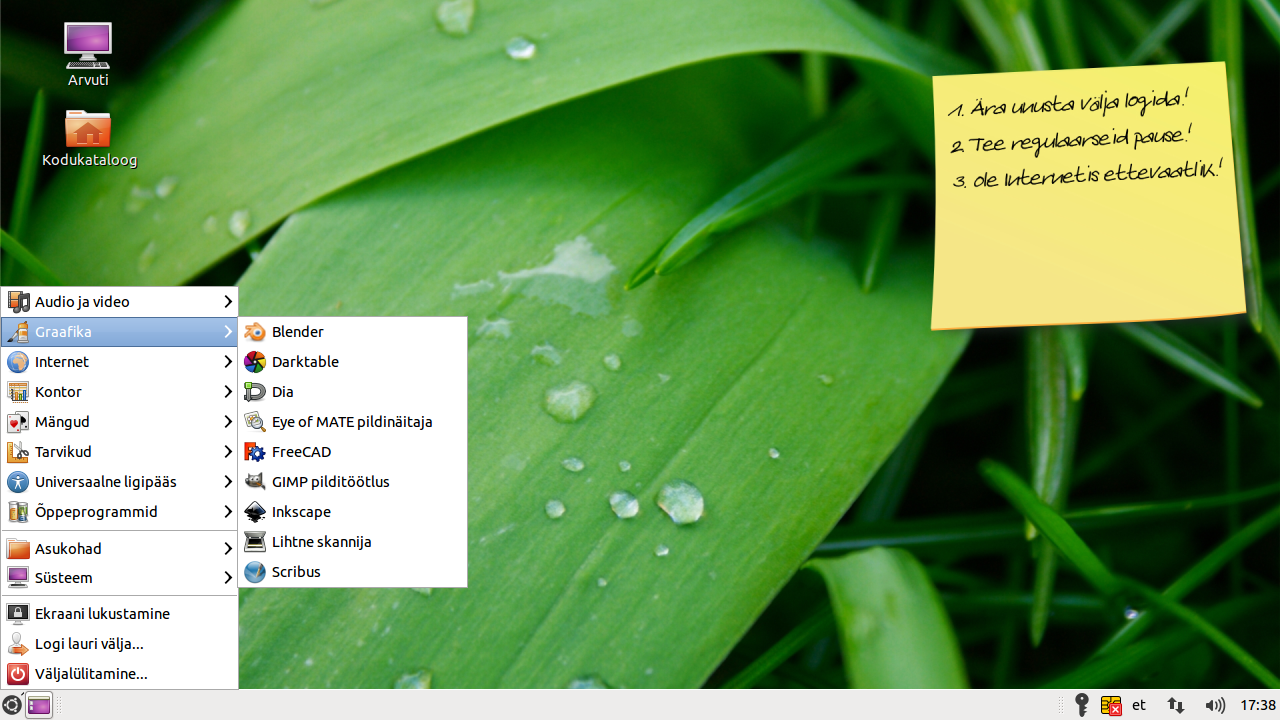
\includegraphics[scale=0.5]{images/edu-workstation}}
\caption{MATE desktop}
\label{fig:digraph}
\end{figure}

We've fine-tuned MATE to slightly mimic Windows XP layout to provide
familiar looks to older generation of users.

\subsection{Software packages}

In addition to Ubuntu software repositories 
we operate an APT repository of 3.6GB which contains
certain proprietary software components necessary
to ease the usage of various hardware equipment.
The repository also contains patched versions of
open-source software which have been modified to cater the
needs of the customers - for example
ID-card enabling packages for Linux based terminal-server,
which are used by National Library of Estonia.

\subsection{Remote management}

As the Ubuntu is being continously improved it also requires
continous maintenance of the templates provided by the service.
Maintaining a well oiled Linux based workstation
requires extensive knowledge of
how the Linux-based operating system is put together of 
thousands of software components and how they interact with each other.
Occasionally skills to dive into C code are necessary
in order to resolve problems.

The templates we ship are automatically associated with
the Puppet master instance which lets us manage
the configuration of the machines and apply critical security updates.


\subsection{Identity service}

Our customized Ubuntu 14.04 template integrates
well with existing Active Directory deployments
and Windows file shares.
We also provide Active Directory compatible
authenticationa and authorization service
for Windows, Ubuntu and Mac OS X workstations using Samba4.
This service is mainly targeted towards
smaller organizations lacking local
infrastructure and manpower to operate such services,
but still wishing to take advantage of centralized
authentication.

\subsection{ownCloud}

ownCloud
is an open-source project which implements
Dropbox functionality to large extent.
Unlike Dropbox, ownCloud can be deployed
on company's or trusted service provider's servers
seamlessly integrating with existing infrastructure
\cite{deploying-owncloud}.
The ownCloud business model is built around selling
enterprise version of ownCloud which has more features
such as Shibboleth authentication which is used by universities.
\cite{owncloud-closes-2.5-million-usd}
There are synchronization clients available
Ubuntu, Windows, Mac OS X, Android and iPhone
making it possible to easily share photos and documents within
an organization.

\begin{figure}[!htb]
\centering
\scalebox{0.5}{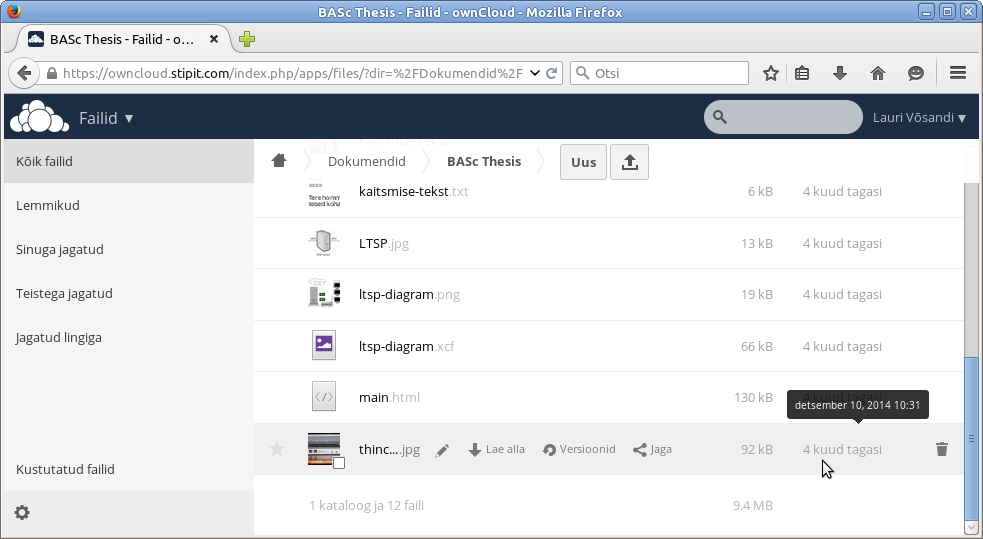
\includegraphics[scale=0.5]{images/owncloud}}
\caption{ownCloud web interface}
\label{fig:digraph}
\end{figure}

For major customers we provide installation,
configuration and maintenance of on-site ownCloud instance.
We also provide shared ownCloud instance
for our customers which is configured to work
in conjunction with our authentication service.
We're planning to add single-sign on
for all the workstations joined to our domain.



\section{Summary}

There is a vast pool of open-source tools available on the Internet
to cater various needs.
Cost to redevelop Linux kernel is estimated to be
approximately \$ 1.4 billion, which is still a fraction
of the development cost of a whole distribution such as Ubuntu
\cite{estimating-cost-of-linux-distro}.
The components are free for use for businesses, governments and
private use, but attention has to be paid to the rights
and obligations implied by a particular license.

There still is very much confusion regarding open-source licenses
and even recognized brands fail to follow the conditions.
For example in VMware was sued in Germany for failure to comply with GPL
\cite{vmware-sued} in March of 2015.
In the past GPL has proven to be effective in court protecting
the authors of the open-source components.

EU has recognized the need to fund open-source projects
mainly due to privacy and security concerns
\cite{eu-should-finance-open-source}.

The companies are starting to see 
software as expense instead of competitive advantage.
\url{http://digitark.ee/eesti-telekom-annab-arisektorile-suunatud-tarkvara-vabakasutusse/}


AVALIKU TEABE SEADUS
avatud riik
open data


\section{Conclusion}

There are various political, economic, societal reasons why
companies and governments wish to use open-source software.
Open-source components significantly decreate time to market
as products can be quickly prototyped and delivered using
readily available components without spending time or finances on
software component producement, licensing or outsourcing.
Nearly all start-ups rely on readily usable open-source
components and modern start-up scene would not be the same
without open-source.

Open-source development model cuts costs and due to
it's deduplicative nature enables pooling of resources 
in order to have better service or product in long run
for all the participants.

%Western world and especially countries of post-soviet syndrome
%have difficulties fully grasping the whole topic and there's
%a lot of misconceptions about open-source and Free Software,
%thus awareness raising is necessary.
%Estonian Free and Open-Source Software Association
%\footnote{\url{http://alvatal.ee/en/}}
%is the corresponding body in Estonia and we have a lot of work to do.

Open-source can be seen as enabling factor for creation of jobs.
Political decisions that foster open-source communities and businesses
also bring increased employment in these sectors,
so cash flow that otherwise would be allocated for
license expenditures
are invested back into local workforce 
pushing the knowledge based society and economics further ahead.

Interestingly the lowest level of resentment for LibreOffice and
Ubuntu was faced in kindergardens,
where computers were not previously used.
For them, the computers were the long needed upgrades
regardless the operating system or office suite.
Thus we highly reccommend for
developing countries to learn from the experience of Baltic countries
and avoid vendor lock-in by building IT infrastructure using
open-source components in the first place
rather than licensing proprietary components
at non-sustainable prices.

The author used the experience gained in the Tallinn migration project
to bootstrap Ubuntu deployment, remote management,
software packaging and ownCloud services.
Software packaging services, Puppet remote management
and earlier version of identity services
are already unrolled to our customers.
Deployment, ownCloud and Samba4 based identity services are in beta testing phase.
The deployment service market launch is planned for 2nd of May as
part of Vabavaratalgud event where Butterknife is
planned to be used to deploy Ubuntu.

We have customers popping up in other market segments such as defence and health care.
We will also continue providing open-source consulting
in various topics: firewalling, virtual private networks,
authentication, authorization, Python programming etc.
Additionally we are co-operating with various e-service providers
such as e-kindergarden to provide up-to-date
Ubuntu OS foundation to consume their web based services.   
Thus is a way we're contributing to the advancement of
standards-compliant web services and innovative usecases
for both public and private sector as standards-compliant
web and multi-platform applications are the enabling factor for
BYOD
\footnote{Bring Your Own Device generally means that instead of
organization provided device the employee is using her own
equipment to work}.

\bibliographystyle{plain}
\bibliography{references}

\end{document}
